\documentclass[12pt, letterpaper]{article}
\usepackage[utf8]{inputenc}
\usepackage{graphicx}
\usepackage{bigints}

\graphicspath{ {image/} } 

\begin{document}

\begin{figure}[h]
	\centering
    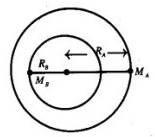
\includegraphics[width = 100px]{two}
\end{figure}

Taking assumptions as in diagram. Applying angular momentum conservation about center of mass:
\begin{equation}
	M_aV_a = M_bV_b
\end{equation}

Using gravitational law:
\begin{equation}
\frac{GM_aM_b}{(r_a + r_b)^2} = M_a\frac{v_a^2}{r_a}
\end{equation}

\begin{equation}
\frac{GM_aM_b}{(r_a + r_b)^2} = M_b\frac{v_b^2}{r_b}
\end{equation}

Assuming circular motion and time period as T, we also have:

\begin{equation}
TV_a = 2\pi r_a
\end{equation}

\begin{equation}
TV_b = 2\pi r_b
\end{equation}

Also,
\begin{equation}
	\frac{2\pi}{T} = \frac{V_a}{r_a} = \frac{V_b}{r_b}
\end{equation}

Putting (6) in (2) and (3). Then using (4), (5) to get rid of $r_a,r_b$. We finally get:


\begin{equation}
M_a = \frac{V_a(V_a+V_b)^2 T}{2 \pi G}
\end{equation}

\begin{equation}
M_b = \frac{V_b(V_a+V_b)^2 T}{2 \pi G}
\end{equation}

\end{document}






